% Inbuilt themes in beamer
\documentclass{beamer}

% Theme choice:
\usetheme{Dresden}
\usecolortheme{whale}

% packages
%\usepackage[hmargin=2cm, vmargin=2cm]{geometry}
\usepackage{microtype}
\usepackage{adjustbox}
\usepackage{graphicx}
\usepackage{hyperref}
\usepackage[english]{babel}
\usepackage{setspace}
%\usepackage{xcolor}
\usepackage{multicol}
\usepackage{float}
\usepackage{amsmath}
\usepackage{amssymb}
\usepackage[font=small,skip=2pt]{caption}
\captionsetup[figure]{labelformat=empty}
\usepackage[
backend=biber,
style=authoryear-comp,
]{biblatex}

\addbibresource{../RMbibliography.bib}
\parindent=0pt

 \newcommand{\independent}{\perp\!\!\!\!\perp} 

% Title page details: 
\title{Scalar on Function Regression \\
with Applications to Near-Infrared Spectroscopy}
\author{Jonathan Willnow, Jakob Juergens, Jonghun Baek}
\date{18.01.2022}

\begin{document}
	
	% Title page frame
	\begin{frame}
		\titlepage 
		\begin{center}
			{\small
			Research Module in Econometrics and Statistics \\
			Winter Semester 2021/2022}
		\end{center}
	\end{frame}
	
	% Remove logo from the next slides
	\logo{}
	
	\begin{frame}{Introduction}
		\textbf{Near-Infrared} (NIR) \textbf{Spectroscopy} enables fast diagnostics by using the NIR region of the electromagnetic spectrum
		\begin{itemize}
			\item Spectroscopy results in high-dimensional dataset: Gasoline dataset (60 x 401)
			\item This set of measurements serves as set of discretized approximations of smooth spectral curves
		\end{itemize}
		\vspace{0.1cm}
		$$\{x_{i}(t_{j,i}) \in \mathbb{R} \: \vert \: i = 1,2,...,N, \; j = 1,2,..., J_i, \; t_{j,i} \in [T_1, T_2] \}$$
	
		\begin{itemize}
			\item Continuous underlying process where $x_i(t)$ exists $\forall t \in [T_1, T_2]$ but is only observed at $t_{j,i}$
			\item Regression to determine relationship between octane rating and spectral curves
		\end{itemize}
		
	\end{frame}

	 \begin{frame}{Random Function}
		A \textbf{Random Variable} is a function $X : \Omega \rightarrow
		\mathcal{S}$ which is defined on a common probability space $(\Omega,
		\mathcal{F}, \mathbb{P})$ where $\Omega$ is a probability space with a
		$\sigma$-algebra $\mathcal{F}$ and a probability measure $\mathbb{{P}}.$
		\vspace{0.2cm}
		
		\begin{itemize}
			\item If $\mathcal{S} = \mathbb{R}$ then $X$ is a random variable
			\item If $\mathcal{S} = \mathbb{R}^{n}$ then $X$ is a random
			vector
			\item If $\mathcal{S}$ is a space of functions, $X$ is called a
			\textbf{Random Function}
		\end{itemize}
		\vspace{0.2cm}
		
		A \textbf{Realization} of a random function $X(\omega)$ is a function 
		$$x_0(t) = X(\omega_0)(t) \quad t \in \mathbb{E}, \: \omega_0 \in \Omega$$
	\end{frame}
	
	\begin{frame}{Plots}
		\begin{minipage}{.5\textwidth}
			\begin{figure}
				
				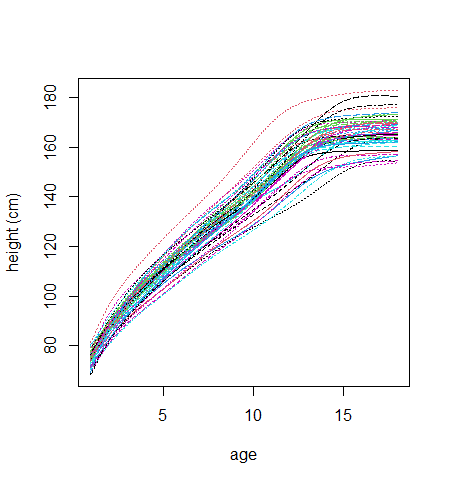
\includegraphics[width=\textwidth]{../Graphics/Growth_curves.png}
				\caption{Growth curves of \\ 54 girls age 1-18}
			\end{figure}
		\end{minipage}%
		\begin{minipage}{.5\textwidth}
			\begin{figure}
				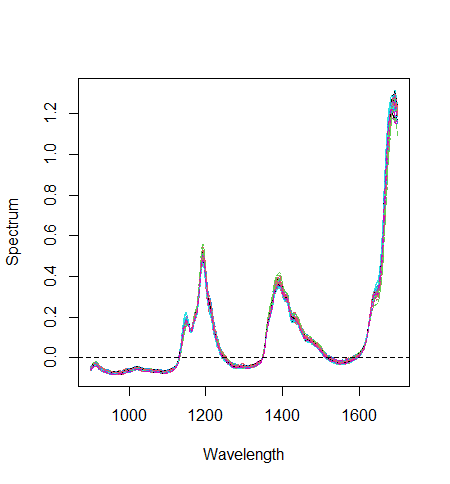
\includegraphics[width=\textwidth]{../Graphics/NIR.png}
				\caption{NIR spectrum of 60 \\ gasoline samples}
			\end{figure}
		\end{minipage}
	\end{frame}
	
	\begin{frame}{Square Integrable Function}
		A function is called \textbf{Square Integrable} written $f(t) \in \mathbb{L}^{2}[0,1]$ if
		$$\int_{0}^{1} \left(f(t)\right)^{2}dt < \infty$$

		\begin{itemize}
			\item Without loss of generality, the interval is defined in $[0,1]$.
		\end{itemize}
		\vspace{0.2cm}
		
		Let $f, g \in \mathbb{L}^{2}[0,1]$, then we can define inner product by
		$$\langle f,g \rangle = \int_{0}^{1} f(t)g(t)dt$$
		
		\begin{itemize}
			\item Orthogonality of two different functions with $\langle f,g\rangle = 0$
		\end{itemize}
	\end{frame}
	
	\begin{frame}{Square Integrable Function}
		A natural \textbf{Norm} to be defined on $\mathbb{L}^2[0,1]$ is the following norm induced by the inner product.
		$$\vert\vert f \vert\vert = \sqrt{\langle f,f \rangle} = \sqrt{\int_{0}^{1} f(t)^2 dt}$$
		\vspace{0.2cm}
		
		This norm naturally induces a \textbf{Distance} on $\mathbb{L}^2[0,1]$.
		$$d(f,g) =  \vert\vert f - g \vert\vert= \sqrt{\langle f-g, f-g \rangle} = \sqrt{\int_{0}^{1} \left[f(t) - g(t)\right]^2 dt}$$
	
	\end{frame}
	
	\begin{frame}{Basis Expansion}
		\textbf{Basis Expansion} is a linear combination of functions as
		described:
		
		$$x_{i}(t) = \sum_{j \in \mathcal{I}} c_{i,j}\phi_{j}(t) \approx
		\sum_{j=1}^{L} c_{i, j}\phi_{j}(t), \quad i = 1, \dots, n, \quad \forall t \in
		\mathbb{E}$$
		
		where $\phi_{j}(t)$ is the $j^{th}$ basis function of the expansion
		and $c_{i, j}$ is the corresponding coefficient. We truncate the basis at $L$
		to:
		\vspace{0.2cm}
		
		\begin{itemize}
			\item make the function smoother
			\item replace the original curves $x_{i}(t)$ with a smaller
			collection of $c_{n, m}$
		\end{itemize}     
	\end{frame}
	
	\begin{frame}{Basis Functions}
		\textbf{Fourier Basis Functions} are elements of the set:
		$$\{\sqrt{2}\sin(2\pi nx) | n \in \mathbb{N}\} \cup
		\{\sqrt{2}\cos(2\pi nx) | n \in \mathbb{N}\} \cup \{1\}$$
		\vspace{-0.5cm}
		\begin{figure}
			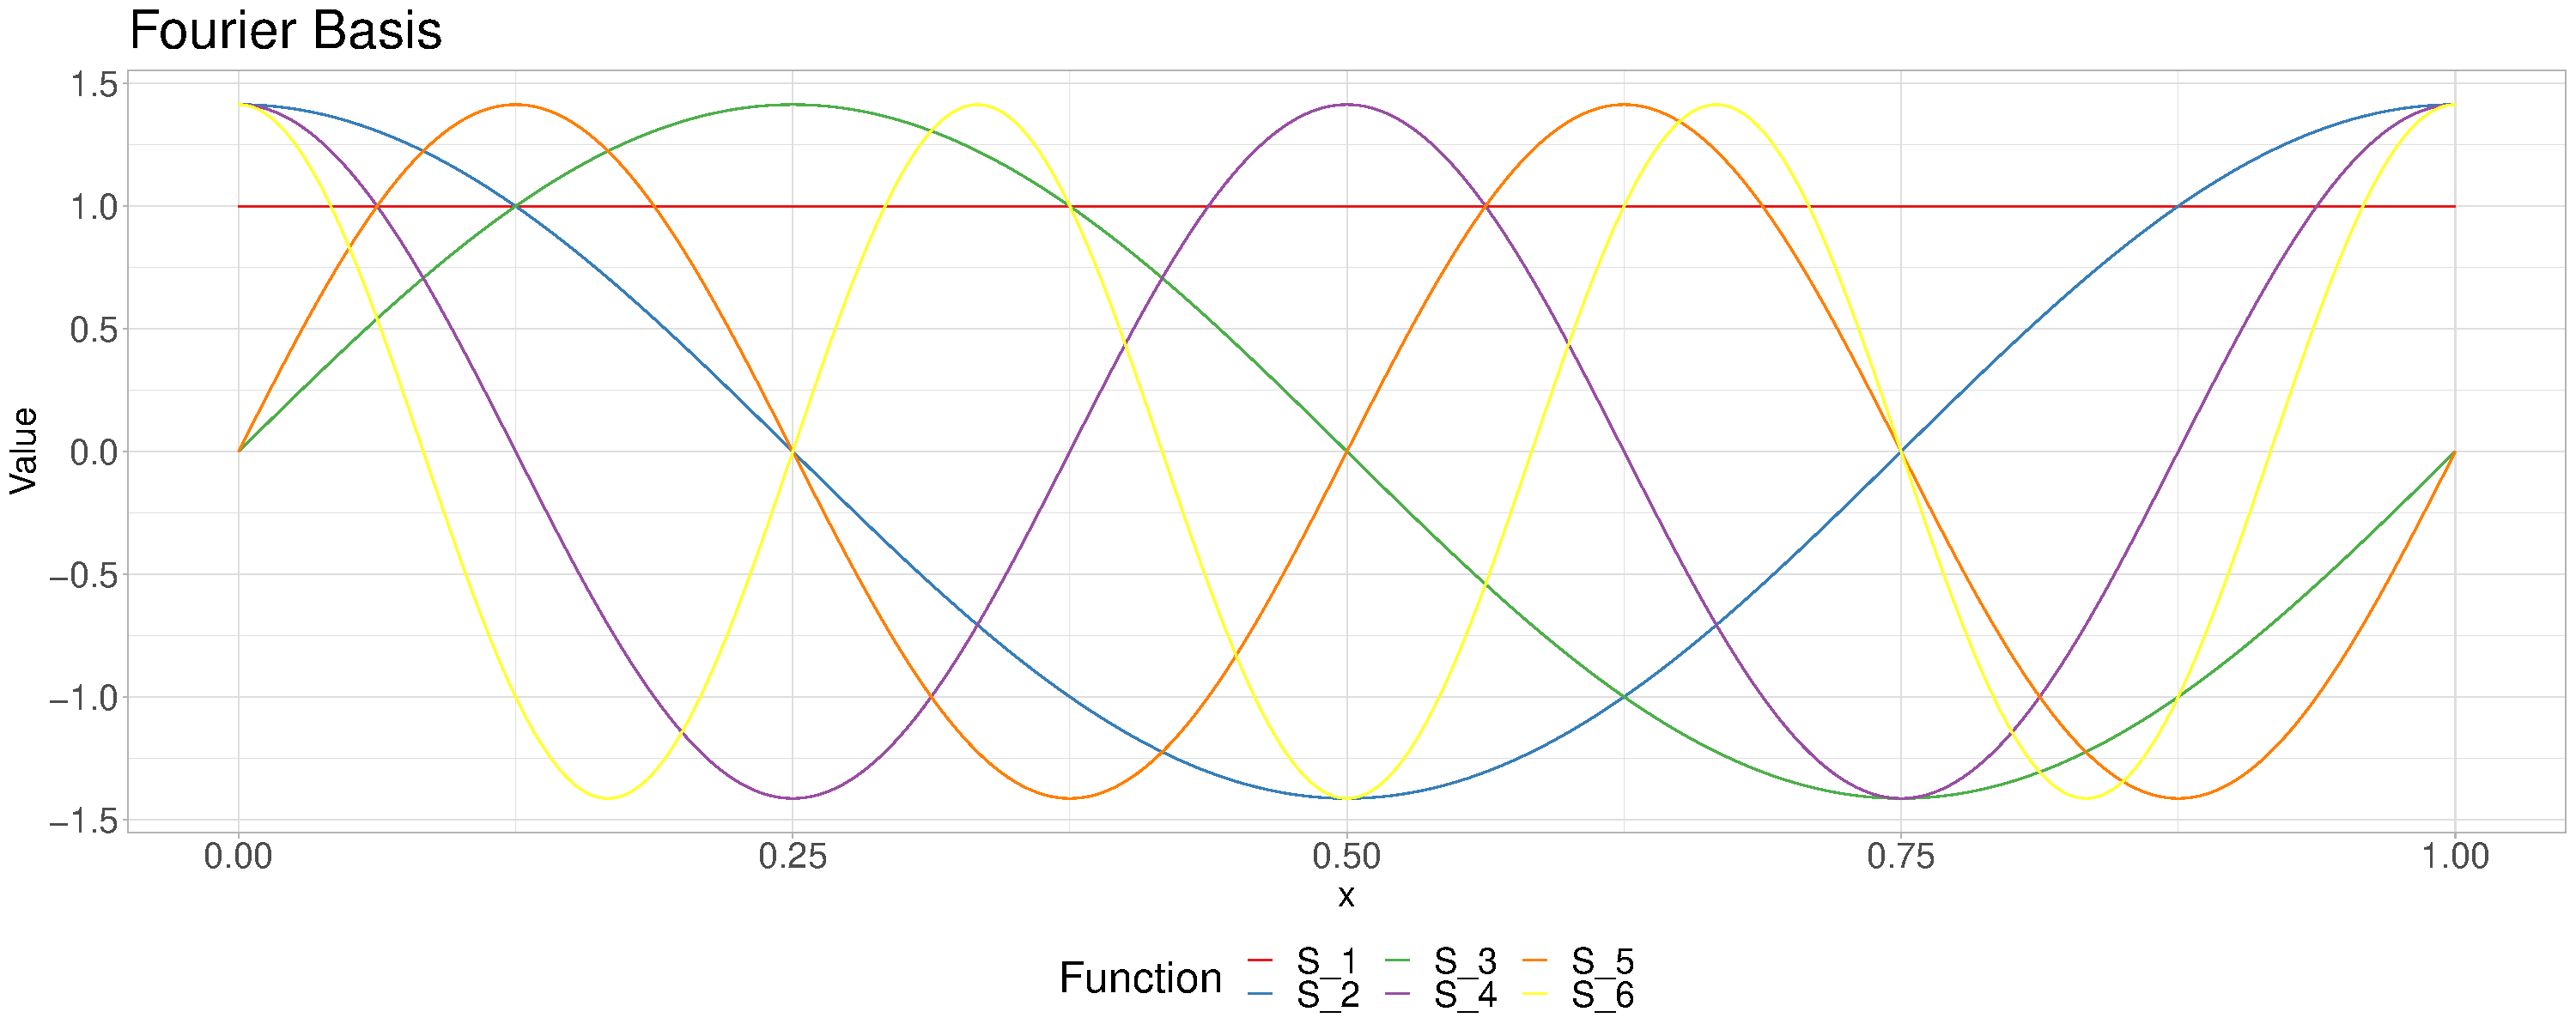
\includegraphics[width =
			\textwidth]{../Graphics/Fourier_Basis.pdf}
			%\caption {Fourier basis functions}
		\end{figure}
		
	\end{frame}
	
	\begin{frame}{Basis Functions}
		\textbf{B-spline Basis Functions} are piece-wise polynomial functions defined by
		an order and a set of knots.
		\begin{figure}
			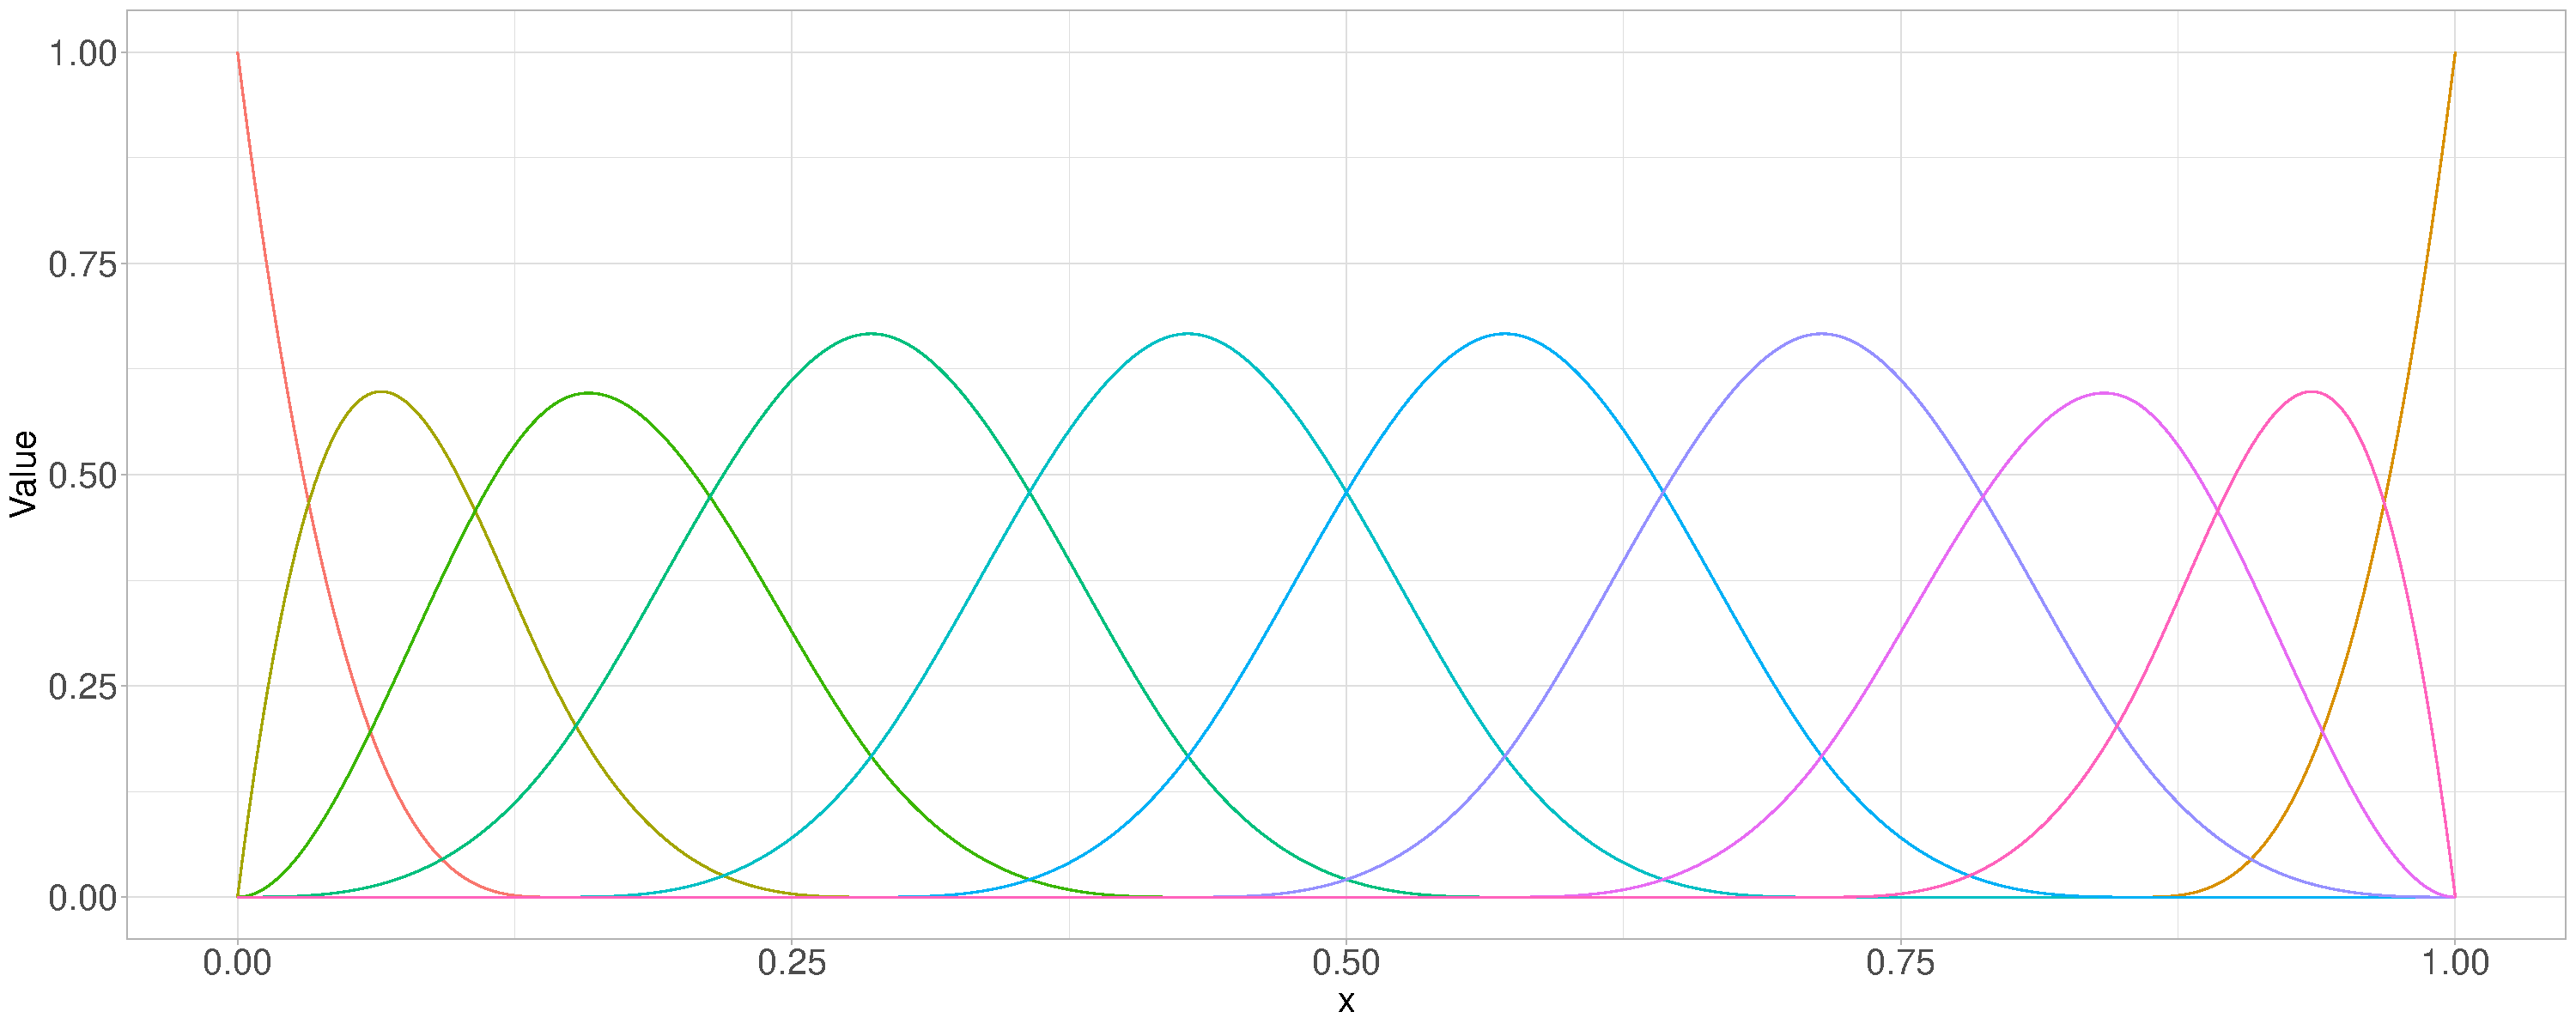
\includegraphics[width =
			\textwidth]{../Graphics/Bspline_Basis.pdf}
			%\caption {Bspline basis functions}
		\end{figure}
	\end{frame}
	
	\begin{frame}{Trade Off between Bias and Variance}
		How do we choose the number $L$ of basis functions?
		
		$$\textbf{MSE}[\hat{X}(t)] = \textbf{Bias}^2[\hat{X}(t)] +
		\textbf{Var}[\hat{X}(t)]$$
		
		$$\textbf{IMSE}[\hat{X}] = \int_{0}^{1} \textbf{MSE}[\hat{X}(t)] dt$$
		
		\begin{itemize}
			\item The larger $L$, the better the fit to the data, but also more fitting noise
			\item If $L$ is too small, the expansion would miss some significant information
		\end{itemize}
	\end{frame}
	
	\begin{frame}{Trade Off between Bias and Variance}
		\begin{figure}\notag
			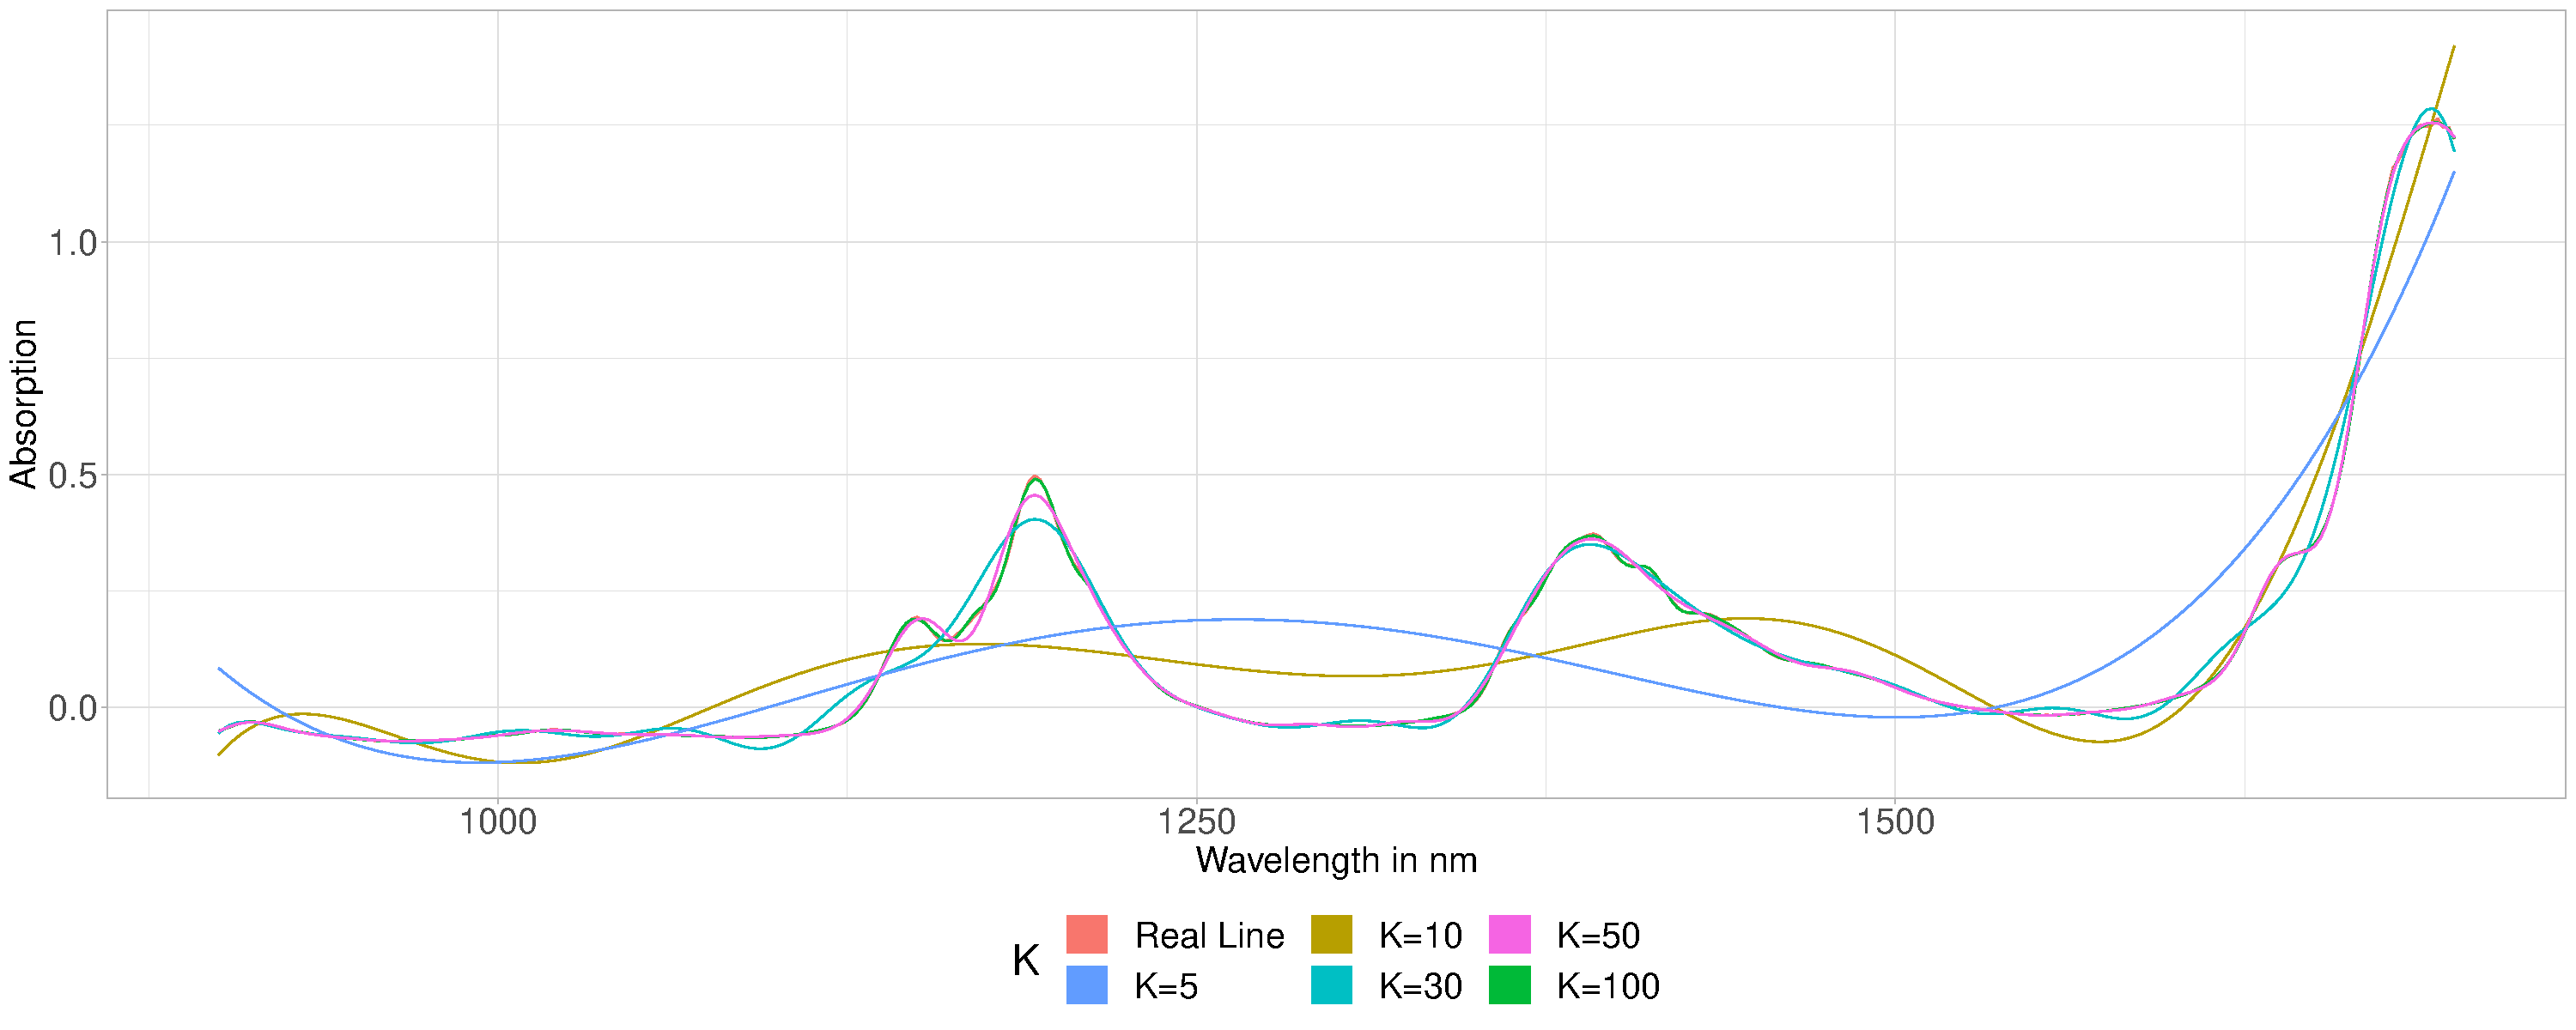
\includegraphics[width =
			\textwidth]{../Graphics/basis_expansions.pdf}
		\end{figure}
	\end{frame}

	\begin{frame}{Estimation via Basis Representation}
		Assume the following \textbf{Data Generating Process}
		$$Y(\omega) = \alpha + \int_{0}^{1} \beta(s) X(\omega)(s) \mathrm{d}s + \epsilon(\omega)$$
		\vspace{-0.6cm}
		\begin{itemize}
			\item $Y(\omega)$ and $\epsilon(\omega)$ realize in $\mathbb{R}$ and $X(\omega)$ realizes in $\mathbb{L}^2[0,1]$
		\end{itemize}
		\vspace{0.7cm}
					
		Let $\{\phi_i(t) \: \vert \: i \in \mathcal{I}\}$ be a basis leading to the following representation
		
		$$\beta(t) = \sum_{j \in \mathcal{I}} c_j \phi_j(t) \approx \sum_{j = 1}^{L} c_j \phi_j(t)$$

	\end{frame}

	\begin{frame}{Estimation via Basis Representation}
		We can transform the data generating process into:
		\begin{equation}\notag
			\begin{split}
				Y(\omega) & = \alpha + \int_{0}^{1}\left[\left(\sum_{j \in \mathcal{I}} c_j  \phi_j(s)\right) X(\omega)(s) \right]\mathrm{d}s + \epsilon(\omega) \\
						  & = \alpha + \sum_{j \in \mathcal{I}} \left[c_j \textcolor{red}{\int_{0}^{1} X(\omega)(s) \phi_j(s)\mathrm{d}s}\right] + \epsilon(\omega)	 \\
						  & = \alpha + \sum_{j \in \mathcal{I}} c_j {\color{red}Z_j(\omega)} + \epsilon(\omega)  \approx  \alpha + \sum_{j = 1}^{L} c_j {\color{red}Z_j(\omega)}  + \epsilon(\omega)
			\end{split}
		\end{equation}
	
		Where a $Z_j(\omega)$ is a \textbf{scalar random variable}.
	\end{frame}

	\begin{frame}{Estimation via Basis Representation}
		Truncating the functional basis allows us to estimate coefficients using \textbf{Multivariate Regression} leading to an estimated coefficient vector $\hat{c} \in \mathbb{R}^L$ and an estimated coefficient function $\hat{\beta}_L(t)$:
		\vspace{-0.2cm}
		$$\hat{\beta}_L(t) = \sum_{j = 1}^{L} \hat{c}_{L,j} \phi_j(t)$$
		
		This is dependent on...\vspace{-0.2cm}
		\begin{multicols}{2}
			\begin{itemize}
				\item The basis $(\phi_j(t))_{j \in \mathcal{I}}$ for the estimation of $\beta(t)$
				\item The truncation parameter $L$\vfill\null
				\item The basis $(\psi_j(t))_{j \in \mathcal{L}}$ used for the observations
				\item The truncation parameter for the observations $K$
			\end{itemize}
		\end{multicols}

	\end{frame}

	\begin{frame}{Karhunen-Lo\'{e}ve Expansion}
		
		\textbf{Mean Function}: $$\mu(t) = \mathbb{E}\left[ X(\omega)(t) \right]$$

		\textbf{Autocovariance Function}: $$c(t,s) = \mathbb{E}\big[ \left( X(\omega)(t) - \mu(t) \right) \left( X(\omega)(s) - \mu(s) \right) \big]$$
		
		The \textbf{Eigenvalues} and \textbf{Eigenfunctions}: $\{(\lambda_i, \nu_i) \: \vert \: i \in \mathcal{I}\}$  are solutions of the following equation:
		$$ \int_{0}^{1}c(t,s)\nu(s) \mathrm{d}s = \lambda \nu(t) $$
	\end{frame}
	
	\begin{frame}{Karhunen-Lo\'{e}ve Expansion}\label{KLE}
		A random function $X(\omega)$ can be expressed in terms of its \textbf{Mean Function} and its \textbf{Eigenfunctions}:
		$$X(\omega)(t) = \mu(t) + \sum_{j = 1}^{\infty} \xi_j(\omega) \nu_j(t)$$
		
		Where the $\xi_j$ are \textbf{Scalar-Valued Random Variables} with the following properties.
		\begin{multicols}{2}
			\begin{enumerate}
				\item $\mathbb{E}[\xi_i(\omega)] = 0$
				\item $Var(\xi_i(\omega)) = \lambda_i$
				\item $Cov(\xi_i(\omega), \xi_j(\omega)) = 0$ for $i \neq j$
			\end{enumerate}
		\end{multicols}
		
		This is called the \textbf{Karhunen-Lo\'{e}ve Expansion} of $X(\omega)$ and the Eigenfunctions can serve as a basis. \\
		
		\hyperlink{spectral}{\beamergotobutton{Spectral Representation of Random Vectors}}
	\end{frame}

	\begin{frame}{Functional Principal Component Analysis}
		\textbf{Principal Component Analysis} can be extended to functional regressors in the form of \textbf{Functional Principal Component Analysis} (FPCA).
		\vspace{0.4cm}
		
		\textbf{Empirical Mean Function}:
		$$\hat{\mu}(t) = \frac{1}{n}\sum_{j = 1}^{n}x_j(t)$$

		\textbf{Empirical Autocovariance Function}:
		$$\hat{c}(t,s) = \frac{1}{n} \sum_{j = 1}^{n} \left(x_j(t) - \hat{\mu}(t)\right) \left(x_j(s) - \hat{\mu}(s)\right)$$

	\end{frame}

	\begin{frame}{Functional Principal Component Analysis}\label{FPCA}
	
		The \textbf{Eigenvalues} and \textbf{Eigenfunctions}: $\{(\hat{\lambda}_i, \hat{\nu}_i) \: \vert \: i \in \mathcal{I}\}$  are solutions of the following equation:
		$$ \int_{0}^{1}\hat{c}(t,s)\hat{\nu}(s) \mathrm{d}s = \hat{\lambda} \hat{\nu}(t) $$
		\vspace{0.2cm}
		
		The $\{\hat{\nu}_i(s) \: \vert \: i \in \mathcal{I}\}$ are called \textbf{Functional Principal Components} and can serve as a basis for representing the original curves. 
		\vspace{0.2cm}
		
		The corresponding scores $\hat{\xi}_i$ can be derived as
		$$\hat{\xi}_j(\omega) = \int_{0}^{1} (F(\omega)(s) - \hat{\mu}(s)) \hat{\nu}_j(s) \mathrm{d}s$$
		
		\hyperlink{PCA}{\beamergotobutton{PCA for Random Vectors}}
	\end{frame}

	\begin{frame}{Simulation Setup}
		Use the \textbf{Gasoline Dataset} (NIR-spectroscopy, 60 $\times$ 401) to generate \textbf{Similar Curves}:
	
		$$\tilde{X}(\omega)(t) = \hat{\mu}(t) + \sum_{j = 1}^{J} \tilde{\xi}_j(\omega) \hat{\nu}_j(t)$$ 
		\vspace{0.2cm}
		
		\begin{itemize}
			\item $\tilde{\xi}_{j} \sim \mathcal{N}(0,\hat{\lambda}_j)$ and $\tilde{\xi}_{j} \independent \tilde{\xi}_{k}$ for $j \neq k$
			\item Simplification: the $\xi_{j}$ do not follow a normal distribution
			\item $\tilde{X}(\omega)(t)$, $\hat{\mu}(t)$ and $\hat{\nu}_j(t)$ are approximated as vectors in $\mathbb{R}^{401}$
		\end{itemize}
		
	\end{frame}
	
	
	\begin{frame}{Simulation Setup cont.}

		Following \textbf{Reiss and Ogden (2007)}, let $f_1(t)$ and $f_2(t)$ be two coefficient functions: 

		\vspace{0.1cm}
		\begin{figure}
			\centering
			\begin{minipage}{.5\textwidth}
				\centering
  				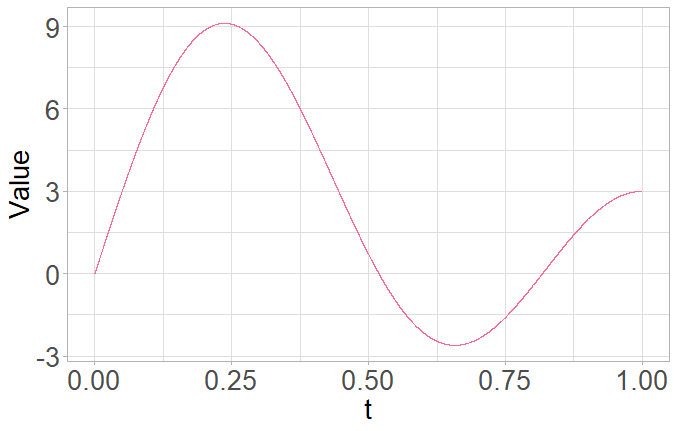
\includegraphics[width=\textwidth]{smooth_function.png}
  				\caption{$f_1(t)$, smooth function}
  				\label{fig:test1}
			\end{minipage}%
			\begin{minipage}{.5\textwidth}
	  			\centering
  				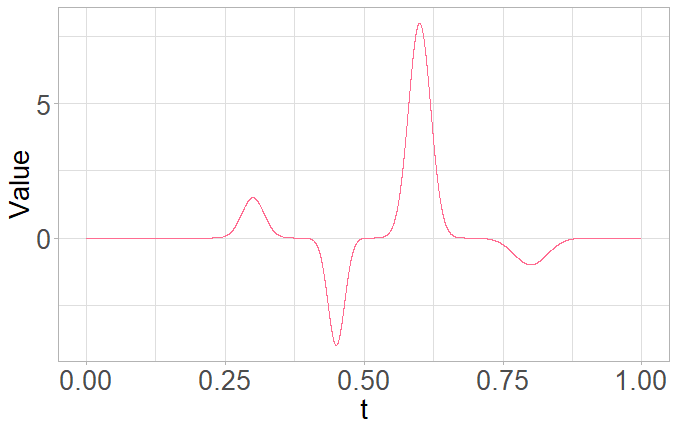
\includegraphics[width=\textwidth]{bumpy_function.png}
  				\caption{$f_2(t)$, bumpy function}
  				\label{fig:test2}
			\end{minipage}
		\end{figure}
		
	\end{frame}	

	
	\begin{frame}{Simulation Setup cont.}
		$$Y_{1,f} = \langle NIR, f\rangle + Z\left(  \frac{var(\langle NIR, f\rangle)}{0.9} - var(\langle NIR, f\rangle)\right)$$ 
		$$Y_{2,f} = \langle NIR, f\rangle + Z\left( \frac{var(\langle NIR, f\rangle)}{0.6} - var(\langle NIR, f\rangle)\right)$$
		
		Let these be two responses for $f \in \{f_1(t), f_2(t)\}$ with $Z \sim \mathcal{N}(0,1)$.	
		\vspace{0.2cm}
		
		\begin{itemize}
    		\item Four combinations with different number of cubic bspline basis-function $n_{basis} \in \{4,5, \dots ,25\}$ and fourier functions $\{1,3, \dots, 25\}$ to perform regression using basis expansion and the FPCR approach.
			\item Compare results via criteria (CV, Mallows CP, ...)
		
		\end{itemize}
	\end{frame}
	
	\begin{frame}{Simulation - Interpretation of Results}\label{Results}
		\textbf{Basis Expansion Regression}
		\begin{itemize}
    			\item Smooth true coefficient functions requires smaller number of $n_{basis}$ and vice versa
    			\item Setup with higher noise requires smoother function.
    			\item  Bspline setup performs overall a bit better.
		\end{itemize}
	
		\textbf{FPCR}
    	\begin{itemize}
    		\item Two PC enough to explain variation.
    		\item Results quite similar, but bspline setup better for smooth function with noisy response.
    	\end{itemize}
    
    	Overall, fourier setup has lower complexity.
    	
    	\hyperlink{Simulation}{\beamergotobutton{Basis Expansion Results}}
    	\hyperlink{Simulation2}{\beamergotobutton{FPCR Results}}
	\end{frame}

	\begin{frame}{Application Setup}
		\begin{itemize}
			\item Use insights from the simulation study to uncover dependence.
			\item Similar setup, but using only bspline basis expansion and initial 60 spectral curves.
			\item Validation set approach:	Scores of test data needs to be estimated by the training data. 
			\item Report results by MSE scaled by variance.
		\end{itemize}
	\end{frame}
	
	\begin{frame}{Further Reading}
		\nocite{hsing_theoretical_2015}
		\nocite{kokoszka_introduction_2017}
		\nocite{Bohacs_Ovadi_Salgo1998}
		\nocite{FR_li_et_al_2020} 
		\nocite{Reiss_2007b}
		\nocite{ramsay_functional_2005}
		\AtNextBibliography{\tiny}
		\printbibliography[heading=none]
	\end{frame}
	
	% From here on out are the supplementary slides.
	
	\begin{frame}{Spectral Representation of Random Vectors}\label{spectral}
		Let $X(\omega)$ be a random vector realizing in $\mathbb{R}^p$.
		
		\begin{itemize}
			\item Let $\mu_x = \mathbb{E}(X)$ and $\Sigma_X = Cov(X)$
			\item Let $\{\gamma_i \: \vert \: i = 1, \dots, p\}$ be the orthonormal \textbf{Eigenvectors} of $\Sigma_X$
			\item Let $\{\lambda_i \: \vert \: i = 1, \dots, p\}$ be the corresponding \textbf{Eigenvalues} of $\Sigma_X$
		\end{itemize}
		
		\vspace{0.2cm}
		Then $X$ can also be represented as
		$$X(\omega) = \mu_x + \sum_{i = 1}^{p} \xi_i(\omega) \gamma_i$$
		where the $\xi_i(\omega)$ have the following properties
		
		\begin{multicols}{2}
			\begin{enumerate}
				\item $\mathbb{E}[\xi_i(\omega)] = 0$
				\item $Var(\xi_i(\omega)) = \lambda_i$
				\item $Cov(\xi_i(\omega), \xi_j(\omega)) = 0$ for $i \neq j$
			\end{enumerate}
		\end{multicols}
	
		\hyperlink{KLE}{\beamergotobutton{Karhunen-Lo\'{e}ve Expansion}}
	\end{frame}

	\begin{frame}{Principal Component Analysis}\label{PCA}
		A related concept is \textbf{Principal Component Analysis} (PCA).
		\vspace{0.2cm}
		
		$\Sigma_X$ unknown $\rightarrow$ \textbf{sample analogues}
		
		\begin{itemize}
			\item Let $\mathbf{X} \in \mathbb{R}^{n \times p}$ contain the standardized regressors
			\item Let $\hat{\Sigma}_X = \frac{\mathbf{X}'\mathbf{X}}{n}$
			\item Let $\{\hat{\gamma}_i \: \vert \: i = 1, \dots, p\}$ be the orthonormal \textbf{Eigenvectors} of $\hat{\Sigma}_X$
			\item Let $\{\hat{\lambda}_i \: \vert \: i = 1, \dots, p\}$ be the corresponding \textbf{Eigenvalues} of $\hat{\Sigma}_X$
		\end{itemize}
		\vspace{0.2cm} 
		
		Then $Z_i(\omega) = \hat{\gamma}_i' X(\omega)$ is called the i'th principal component and
		\begin{multicols}{2}
			\begin{enumerate}
				\item $\mathbb{E}[Z_i(\omega)] = 0$
				\item $Var(Z_i(\omega)) = \hat{\lambda}_i$
				\item $Cov(Z_i(\omega), Z_j(\omega)) = 0$ for $i \neq j$
			\end{enumerate}
		\end{multicols}
		\hyperlink{FPCA}{\beamergotobutton{Functional Principal Component Analysis}}
	\end{frame}

	\begin{frame}{Simulation Results - bspline basis expansion}\label{Simulation}
		\begin{table}
			\centering
			\resizebox*{\columnwidth}{!}{%
				\begin{tabular}{lllllll}
					\cline{2-6}
					& \textbf{f1\_e1\_spline}                 & \textbf{f1\_e2\_spline}                 & \textbf{f2\_e1\_spline}                   & \textbf{f2\_e2\_spline}                 & \textbf{n\_basis} &  \\ \cline{2-6}
					& 2.1318                        & {\color[HTML]{FE0000} 71.71} & 0.6082                        & 1.5345                        & 4                &  \\
					& 2.0076                        & 71.9395                      & 0.3427                        & 1.2906                        & 5                &  \\
					& {\color[HTML]{FE0000} 1.9937} & 72.2563                      & 0.2456                        & 1.2014                        & 6                &  \\
					& 2.0365                        & 73.7857                      & 0.2797                        & 1.2495                        & 7                &  \\
					& 2.1861                        & 79.0485                      & 0.1044                        & 1.1458                        & 8                &  \\
					& 2.0511                        & 74.1784                      & 0.0356                        & {\color[HTML]{FE0000} 1.0217} & 9                &  \\
					& 2.1052                        & 76.1884                      & 0.0297                        & 1.0393                        & 10               &  \\
					& 2.1012                        & 76.4031                      & {\color[HTML]{FE0000} 0.0296} & 1.0425                        & 11               &  \\
					& 2.3815                        & 86.1707                      & 0.037                         & 1.1819                        & 12               &  \\
					& 2.2114                        & 80.6208                      & 0.0363                        & 1.1024                        & 13               &  \\
					& 2.4495                        & 87.6977                      & 0.038                         & 1.2126                        & 14               &  \\
					& 2.2887                        & 83.4755                      & 0.0315                        & 1.1363                        & 15               &  \\
					& 2.5491                        & 93.593                       & 0.0352                        & 1.2652                        & 16               
				\end{tabular}%
			}
		\end{table}
		\hyperlink{Results}{\beamergotobutton{Results}}
	\end{frame}
	
	
	
	\begin{frame}{Simulation Results - fourier basis expansion}
		\begin{table}
			\centering
			\resizebox*{\columnwidth}{!}{%
				\begin{tabular}{lllllll}
					\cline{2-6}
					& \textbf{f1\_e1\_spline}                 & \textbf{f1\_e2\_spline}                 & \textbf{f2\_e1\_spline}                   & \textbf{f2\_e2\_spline}                 & \textbf{n\_basis} &  \\ \cline{2-6}
					& 0                            & 0                              & 0                            & 0                             & 1                &  \\
					& 2.0292                       & {\color[HTML]{FE0000} 72.0085} & 0.512                        & 1.4747                        & 3                &  \\
					& {\color[HTML]{FE0000} 2.022} & 72.6017                        & 0.1616                       & 1.1375                        & 5                &  \\
					& 2.0355                       & 73.1836                        & 0.0293                       & {\color[HTML]{FE0000} 0.9907} & 7                &  \\
					& 2.062                        & 73.9631                        & {\color[HTML]{FE0000} 0.029} & 0.9994                        & 9                &  \\
					& 2.0881                       & 75.0921                        & 0.0291                       & 1.0139                        & 11               &  \\
					& 2.0997                       & 75.9422                        & 0.0294                       & 1.0291                        & 13               &  \\
					& 2.1087                       & 76.7123                        & 0.0298                       & 1.0371                        & 15               &  \\
					& 2.1301                       & 77.4908                        & 0.03                         & 1.0398                        & 17               &  \\
					& 2.1535                       & 78.3943                        & 0.0303                       & 1.0509                        & 19               &  \\
					& 2.1775                       & 79.2058                        & 0.0307                       & 1.0617                        & 21               &  \\
					& 2.2058                       & 80.3801                        & 0.031                        & 1.077                         & 23               &  \\
					& 2.2372                       & 81.509                         & 0.0315                       & 1.0905                        & 25               & 
				\end{tabular}%
			}
		\end{table}
		\hyperlink{Results}{\beamergotobutton{Results}}
	\end{frame}
	
	
	\begin{frame}{Simulation Results - bspline FPCR ($n_{harm}$ = 2)}\label{Simulation2}
		\begin{table}
			\centering
			\resizebox*{\columnwidth}{!}{%
				\begin{tabular}{llllllll}
					\cline{2-7}
					& \boldmath{$f_1$}\textbf{, error 1}                 & \boldmath{$f_1$}\textbf{, error 2}                  & \boldmath{$f_2$}\textbf{, error 1}                    & \boldmath{$f_2$}\textbf{, error 2}                 & \textbf{expl. variance} & \textbf{n\_basis} &  \\ \cline{2-7}
					& 2.9163                       & 10.8768                       & 0.9599                        & 1.6431                        & 1                & 4                &  \\
					& {\color[HTML]{FE0000} 2.345} & {\color[HTML]{FE0000} 10.585} & 0.8649                        & 1.5631                        & 0.9776           & 5                &  \\
					& 2.4187                       & 10.6889                       & 0.8739                        & 1.5759                        & 0.9556           & 6                &  \\
					& 2.4971                       & 10.7287                       & 0.8625                        & 1.5723                        & 0.9472           & 7                &  \\
					& 2.5799                       & 10.6971                       & 0.8716                        & 1.575                         & 0.9239           & 8                &  \\
					& 2.6828                       & 10.7669                       & 0.853                         & 1.5661                        & 0.9178           & 9                &  \\
					& 2.825                        & 10.7906                       & 0.8304                        & 1.5622                        & 0.8976           & 10               &  \\
					& 2.9082                       & 10.7774                       & {\color[HTML]{FE0000} 0.8237} & {\color[HTML]{FE0000} 1.5424} & 0.906            & 11               &  \\
					& 2.9519                       & 10.8126                       & 0.8286                        & 1.5561                        & 0.9036           & 12               &  \\
					& 2.9972                       & 10.8221                       & 0.8404                        & 1.5551                        & 0.9052           & 13               &  \\
					& 2.9755                       & 10.7706                       & 0.8396                        & 1.5614                        & 0.9074           & 14               &  \\
					& 2.9762                       & 10.7946                       & 0.8476                        & 1.557                         & 0.9058           & 15               &  \\
					& 2.9627                       & 10.8067                       & 0.8609                        & 1.5615                        & 0.9061           & 16          
				\end{tabular}%
			}
		\end{table}
		\hyperlink{Results}{\beamergotobutton{Results}}
	\end{frame}
	
	
	
	\begin{frame}{Simulation Results - fourier FPCR ($n_{harm}$ = 2)}
		\begin{table}
			\centering
			\resizebox*{\columnwidth}{!}{%
				\begin{tabular}{llllllll}
					\cline{2-7}
					& \boldmath{$f_1$}\textbf{, error 1}                 & \boldmath{$f_1$}\textbf{, error 2}                  & \boldmath{$f_2$}\textbf{, error 1}                    & \boldmath{$f_2$}\textbf{, error 2}                 & \textbf{expl. variance} & \textbf{n\_basis} &  \\ \cline{2-7}
					& 0                             & 0                              & 0                             & 0                             & 0       & 1       &  \\
					& {\color[HTML]{FE0000} 2.2059} & {\color[HTML]{FE0000} 11.2438} & 0.8768                        & 1.5528                        & 0.9846  & 3       &  \\
					& 2.2148                        & 11.2567                        & {\color[HTML]{FE0000} 0.8227} & {\color[HTML]{FE0000} 1.5215} & 0.9584  & 5       &  \\
					& 2.2635                        & 11.2662                        & 0.8828                        & 1.5563                        & 0.9489  & 7       &  \\
					& 2.2721                        & 11.2692                        & 0.8811                        & 1.5531                        & 0.9439  & 9       &  \\
					& 2.2797                        & 11.2574                        & 0.879                         & 1.555                         & 0.9397  & 11      &  \\
					& 2.3039                        & 11.2708                        & 0.8887                        & 1.5591                        & 0.9421  & 13      &  \\
					& 2.3248                        & 11.2898                        & 0.8743                        & 1.5514                        & 0.9283  & 15      &  \\
					& 2.3798                        & 11.2957                        & 0.875                         & 1.5511                        & 0.9182  & 17      &  \\
					& 2.4233                        & 11.3049                        & 0.8632                        & 1.5453                        & 0.9167  & 19      &  \\
					& 2.4589                        & 11.3094                        & 0.8619                        & 1.5432                        & 0.9133  & 21      &  \\
					& 2.5306                        & 11.331                         & 0.8562                        & 1.5408                        & 0.9082  & 23      &  \\
					& 2.5752                        & 11.3272                        & 0.8531                        & 1.5393                        & 0.9062  & 25      & 
				\end{tabular}%
			}
		\end{table}
		\hyperlink{Results}{\beamergotobutton{Results}}
	\end{frame}
\end{document}